\documentclass[a4paper,12pt]{report}
\usepackage[utf8]{inputenc}
\usepackage[francais]{babel}
\usepackage{fancyhdr}
\usepackage{graphicx}
\usepackage{tikz}
\usetikzlibrary{calc}
\usepackage{listings}
\usepackage{xcolor}
\definecolor{grey}{rgb}{0.9,0.9,0.9}
\usepackage{titlesec}
\usepackage{verbatim}
\usepackage{listings}
\usepackage{textcomp}
\usepackage{hyperref}
\usepackage{longtable}
\usepackage{colortbl}
\usepackage{amssymb}


\frenchbsetup{StandardLists=true}
\newcommand{\marge}{18mm}
\usepackage[left=\marge,right=\marge,top=\marge,bottom=\marge]{geometry}
\pagestyle{fancy}
\setlength{\headheight}{14pt}
\chead{
  \textbf{Monôme:} Douaille Erwan 
    \hspace{2em}
  \textbf{Groupe:} M2 Info IVI}
\renewcommand{\headrulewidth}{1pt}
\linespread{1}
\setlength{\columnseprule}{0.2pt}
\definecolor{javakeyword}{rgb}{0,0,0.5}
\definecolor{javastring}{rgb}{0,0.5,0}
\definecolor{javacomment}{rgb}{0.5,0.5,0.5}
\lstdefinestyle{C++}{
   language=C++, basicstyle=\footnotesize,       % the size of the fonts that are used for the code
  numbers=left,                   % where to put the line-numbers
  numberstyle=\tiny\color{gray},  % the style that is used for the line-numbers
  stepnumber=1,                   % the step between two line-numbers. If it's 1, each line
                                  % will be numbered
  numbersep=5pt,                  % how far the line-numbers are from the code
  backgroundcolor=\color{white},  % choose the background color. You must add \usepackage{color}
  showspaces=false,               % show spaces adding particular underscores
  showstringspaces=false,         % underline spaces within strings
  showtabs=false,                 % show tabs within strings adding particular underscores
  frame=single,                   % adds a frame around the code
  rulecolor=\color{black},        % if not set, the frame-color may be changed on line-breaks within not-black text (e.g. commens (green here))
  tabsize=2,                      % sets default tabsize to 2 spaces
  captionpos=b,                   % sets the caption-position to bottom
  breaklines=true,                % sets automatic line breaking
  breakatwhitespace=false,        % sets if automatic breaks should only happen at whitespace
  title=\lstname,                 % show the filename of files included with \lstinputlisting;
   stringstyle=\color{javastring},
   keywordstyle=\color{javakeyword}\ttfamily\textbf,
   commentstyle=\color{javacomment}\ttfamily\textit
 }
\begin{document}



\makeatletter
\begin{titlepage}
\centering
\vspace{-10em}
{\LARGE \textbf{\textsc{Rapport de Projet RVI}}}\\
\vspace{3em}

\includegraphics[scale=0.6]{image/thalassa.png}\\
\vspace{3em}
{\LARGE \textsc{Projet Thalassa: simulation de plongée sous-marine}}\\

\vspace{8em}
Par\\
\vspace{1em}
{\LARGE \@author}\\

\vspace{2em}



\begin{tikzpicture}[remember picture,overlay]

\node [below left,xshift=-1cm, yshift=4cm] at (current page.south east){
\includegraphics[scale=0.6]{image/ustl1.png}};

\end{tikzpicture}
\end{titlepage}
\makeatother

\sloppy

\setcounter{page}{1} 
\newpage

\section*{Introduction}

Le but de ce TP est de nous faire découvrir une méthode simple d'implémentation de mise en correspondance de points d'intérêts sur des images stéréo. Afin de réaliser cette objectif il nous faudra calculer une matrice fondamentale qui nous permettra d'obtenir les droites épipolaires, ensuite nous chercherons les points d'intérêts et enfin nou calculerons les distances de ces points d'intérêts par rapports aux droites épipolaires ce qui nous permettra la réalisation de la mise en correspondance.


\section*{Calcul de la matrice fondamentale}

La matrice fondamentale est une matrice de type \textit{3x3} qui permet de relier des points dans une image stéréo. Plus concrètement, elle va nous permmettre d'obtenir la droite épipolaire d'un point dans un plan opposée.

Une droite épipolaire est une droite placée dans l'autre image que celle sur laquelle se trouve notre point d'intérêt. L'avantage d'utiliser la géométrie épipolaire est que ces méthodes nous permettent de mettre en correspondance deux images sans connaître l'emplacement des périphériques de capture. 

Pour déterminer la matrice fondamentale il nous faut déterminer une matrice homographie. Cette matrice homographie est calculée dans \textit{iviVectorProductMatrix} et est déterminée selon la formule du cours :

\begin{figure}[!ht]
	\center
	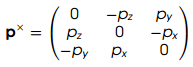
\includegraphics[scale=0.6]{./image/vector.png}
\end{figure}

Pour calculer la matrice fondamentale nous reprennons également la formule du cours: 

\begin{figure}[!ht]
	\center
	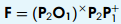
\includegraphics[scale=0.7]{./image/funda.png}
\end{figure}

\textit{(p2*o1)} est notre matrice homographie, p2 et p1 sont des matrices de projections des plan droit et gauche. \textit{p1\up{+}} signifie que l'on souhaite l'inverse de cette matrice de projection.

La matrice fondamentale une fois calculée va nous permettre de déterminer les droites épipolaires qui seront utiles pour la mise en correspondance des points d'intérêts des deux images.

\newpage

\section*{Extraction des coins}

Dans cette partie, notre but est de mettre en évidence des pixels d'intérêts dans les deux images qui serviront à faire une mise en correspondance des images stéréo.

Pour obtenir ces pixels d'intérêts nous allons utiliser une fonction implémentée dans openCV nommée \textit{goodFeaturesToTrack} qui met en application la méthode proposée par \textit{Jianbo Shi} et \textit{Carlo Tomasi}.

Voici un extrait du code obtenu, accompagné d'un descriptif des paramètres de la fonction \textit{goodFeaturesToTrack}:
\begin{lstlisting}[style=C++]
	vector<Point2f> vCorners;
    
    // mImage, image a analyser
    // vCorners, liste qui sera remplit et contiendra les points d'interets
    // iMaxCorners, nombre max de points a determiner
    // 0.01
    // 10
    // La suite des parametres sont des valeurs par defaut utilises pour la methode de calcul de detection des contours de Harris. Harris detector est une autre methode de dectection de points, cf article du cours. La methode de J. Shi and C. Tomasi est une amelioration du detecteur de Harris.
    goodFeaturesToTrack(mImage,vCorners,iMaxCorners,0.01,10,Mat(),3,false,0.04);
    // ... Point2D to Point3D and return
}
\end{lstlisting}

Avec cette méthodes nous avons obtenu une liste de points qui sont apparus sur nos deux images. On remarque que ces points sont les mêmes sur les deux images.

\begin{figure}[!ht]
	\center
	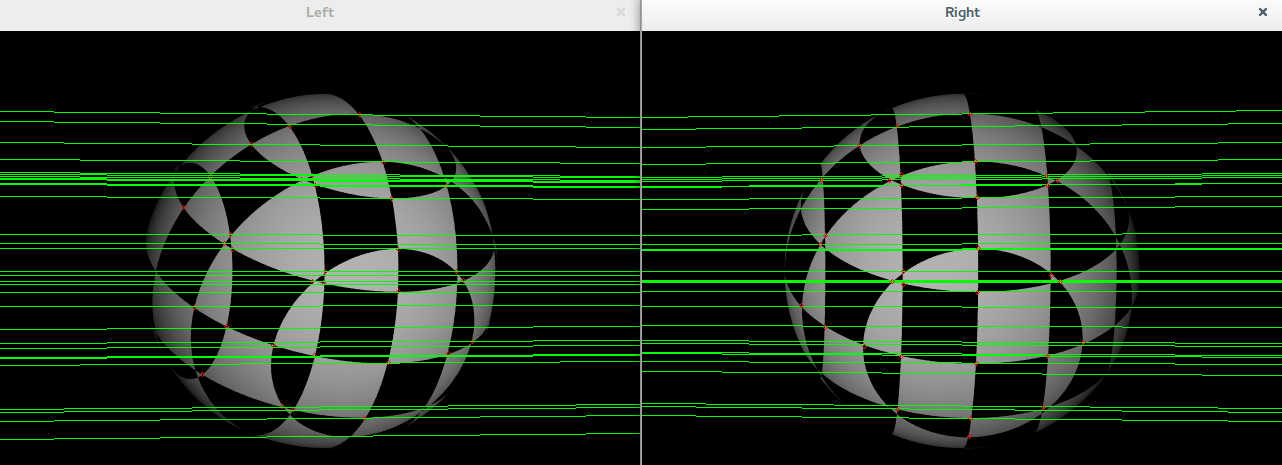
\includegraphics[scale=0.4]{./image/detect-corner.png}
\end{figure}

\begin{figure}[!ht]
	\center
	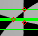
\includegraphics[scale=1]{./image/corner.png}
\end{figure}

On observe en zoomant que des points d'intérêts sont apparus. On peut remarquer sur l'image de gauche qu'une droite en bas de l'image semble ne passer par aucun point. Cette droite est la droite épipolaire associée au point d'intérêt en bas de l'image de droite. On observe bien que cette droite épipolaire passe par le point sur lequel se trouve notre point d'intérêt.

\newpage
\section*{Calcul des distances}

Dans cette section nous avons l'ensemble des points d'intérêts ainsi que les droites épipolaires.

L'objectif de cette partie est de calculer la distance entre un point d'intérêt avec l'ensemble des droite épipolaires dans l'image opposée pour nous permettre par la suite de déterminer la correspondance entre les point d'intérêt de l'image gauche avec l'image droite.

\begin{lstlisting}[style=C++]
 for(int i=0;i<widthLeft;i++){
        Mat pL = m2DLeftCorners.col(i);
        Mat epipolaireL = mFundamental * pL;
        for(int j = 0; j < widthRight; j++) {
            Mat pR = m2DRightCorners.col(j);
            Mat epipolaireR = mFundamental.t() * pR;
            mDistances.at<double>(i,j) = ((abs(epipolaireL.at<double>(0) * pR.at<double>(0) + epipolaireL.at<double>(1) * pR.at<double>(1) + epipolaireL.at<double>(2)))
                                          /(sqrt(pow(epipolaireL.at<double>(0),2) + pow(epipolaireL.at<double>(1),2)))) +

                                        ((abs(epipolaireR.at<double>(0)*pL.at<double>(0)+epipolaireR.at<double>(1)*pL.at<double>(1)+epipolaireR.at<double>(2)))
                                        /(sqrt(pow(epipolaireR.at<double>(0),2) + pow(epipolaireR.at<double>(1),2))));
        }
    }
    return mDistances;
}
\end{lstlisting}

L'idée est de calculer toute les distances d'un point avec l'ensemble des droites épipolaires (comme visible avec les deux boucles for), ce qui nous permettra de déterminer les correspondances des points en cherchant la distance minimum d'une droite et d'un point dans la section suivante.

Pour déterminer comment calculer la distance entre un point et sa droite, nous avons utilisé la formule suivante:

\begin{figure}[!ht]
	\center
	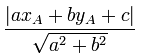
\includegraphics[scale=0.6]{./image/distance.png}
\end{figure}

\textit{a}, \textit{b} et \textit{c} correspondent à \textit{x,y,z} de notre droite épipolaire. \textit{$ x_{a} $, $ y_{a} $} correspondent au \textit{x, y} de notre point d'intérêt. Comme visible dans le code ci-dessus, une fois cette distance calculée on fait la somme des deux distances euclidiennes, celle entre le point de l'image gauche et la droite épipolaire de l'image gauche associée au point de l'image droite et celle entre le point de l'image droite et la droite épipolaire de l'image droite associée au point de l'image gauche.


\newpage

\section*{Mise en correspondance}

À partir de maintenant nous avons une matrice contenant la distance entre tout les points d'une image avec l'ensemble des droites épipolaires présentes dans l'image opposée. À partir de cette matrice il nous est possible de faire la mise en correspondance des points d'intérêts entre les images stéréo.

\textit{iviMarkAssociations} est la méthode dans laquelle nous allons calculer les correspondances, voici un extrait de code pouvant apporter un support aux explications qui vont suivre:


\begin{lstlisting}[style=C++]
 for(int i= 0; i< width ; i++) {
        int min = dMaxDistance;
        int minIndex = -1;
        for(int j= 0; j< height; j++) {
            if(min>mDistances.at<double>(i,j) && mDistances.at<double>(i,j)<dMaxDistance) {
                min = mDistances.at<double>(i,j);
                minIndex = j;
            }
        }
        mRightHomologous.at<double>(i,0) = minIndex;
    }

    for(int i= 0; i< height ; i++) {
        int min = dMaxDistance;
        int minIndex = -1;
        for(int j= 0; j< width; j++) {
            if(min>mDistances.at<double>(j,i) && mDistances.at<double>(j,i)<dMaxDistance) {
                min = mDistances.at<double>(j,i);
                minIndex = j;
            }
        }
        mLeftHomologous.at<double>(i,0) = minIndex;
    }
\end{lstlisting}


L'idée est de parcourir la matrice des distances dans un sens et de regarder la distance minimale sur la colonne ou sur la ligne (dépend du sens de parcours). Une fois le minimum récupéré et inférieur à notre valeur de distance maximale, nous sauvegardons l'index du tableau où est contenue la distance minimale dans le tableau \textit{mLeftHomologous} par exemple. Et nous parcourrons la matrice de distance dans le sens opposé en appliquant le même mécanisme mais en sauvegardant le résultat dans \textit{mRightHomologous}.

Maintenant nous avons une estimation de la correspondance des points de l'image gauche et droite.

Nous avons remarqué que certains points n'ont pas trouvé de correspondant, dûe à la distance de seuil que nous imposons. En effet pour certains points la distance obtenue entre lui-même et une droite épipolaire dans l'image opposée est trop importante et dépasse le seuil maximale que nous impossons. Nous avons remarqué que plus ce seuil est important, plus le nombre de correspondances est important.

En plus de ce problème de distance supérieur au seuil, nous avons constaté qu'il y a des conflits entre certains points.

\begin{figure}[!ht]
	\center
	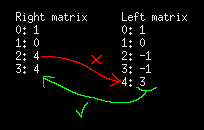
\includegraphics[scale=0.8]{./image/resultincorrect.png}
\end{figure}

Dans l'image ci-dessus (\textit{Right Matrix}) on constate que deux points ont la même correspondance \textit{2 et 3} dans l'image opposée, \textit{Left Matrix}. Ce problème est dûe au fait que certains points sont très proche les uns des autres. De plus comme nous fesons un parcours itératif pour déterminer les correspondances nous ne tenons pas compte des valeurs déterminées précédemments, ce qui donne ce genre de résultats \textit{incohérents}.

\begin{figure}[!ht]
	\center
	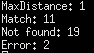
\includegraphics[scale=1]{./image/result.png}
	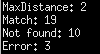
\includegraphics[scale=1]{./image/result2.png}
	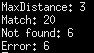
\includegraphics[scale=1]{./image/result1.png}
\end{figure}

Pour une distance de seuil maximale à deux, nous obtenons 19 correspondances, 9 sans correspondances déterminées (en parties dûe à la valeur de seuil) et 4 incohérences. On remarque que plus la valeur maximale de distance augmente, plus il y a de correspondances trouvées. L'augmentation de la valeur maximale augmente également les problémes de matching car cela étend les zones de \textit{recherches} des points correspondants et crée donc plus d'erreur.


\section*{Conclusion}

Pour conclure, dans ce tp nous avons appris à déterminer une matrice fondamentale ainsi qu'à l'utiliser pour déterminer les droites épipolaires qui elles même nous ont permis la mise en correspondance des points d'intérêts. Cela nous à également montré la compléxitée à déterminer des correspondances entre deux images stéréo. Le problème de mise en correspondance de facon itérative montre bien qu'un simple algorithme "\textit{naif}" ne suffit pas à correctement mettre en correspondance des points sur des images différentes.


\end{document}